\documentclass[oneside,a4paper,11pt,explicit]{book}
\usepackage[utf8]{inputenc}
\usepackage{icecream}
\usepackage[english]{babel}
\addto\captionsenglish{\renewcommand{\chaptername}{}}
\usepackage[accsupp]{axessibility}  % improves PDF readability for those with disabilities.
\usepackage[colorlinks = true,urlcolor  = blue,linkcolor = blue]{hyperref}
\usepackage{setspace}
\usepackage{listings}
\usepackage[most]{tcolorbox}
\usepackage{minitoc}


\renewcommand{\mtifont}{\large\sffamily}
\renewcommand{\mtcfont}{\small\sffamily}
\renewcommand{\mtcSfont}{\small\sffamily}
\renewcommand{\mtcSSfont}{\small\sffamily}
\renewcommand{\mtcSSSfont}{\small\sffamily}
\mtcsetpagenumbers{minitoc}{off} % turn off page numbering in minitocs
\addto{\captionsenglish}{% Making babel aware of special titles
	\renewcommand{\mtctitle}{Quick Links To Sections}
}
\setlength{\fboxrule}{5pt}
\setlength{\fboxsep}{4pt}

\definecolor{IceCreamLeaf}{rgb}{0.4, 0.639215686274, 0.4}
\definecolor{IceCreamOrbit}{rgb}{0.803921568627451, 0.3607843137254902, 0.3607843137254902}

\pretolerance=10000
\tolerance=2000 
\emergencystretch=10pt

%%%%%%%%%%%%%%% END PREAMBLE

\title{I.C.E.C.R.E.A.M. Tutorials}
\subtitle{\small Observing Earth from Above (Env 329) v24.06  \\
	\small Schmid College of Science and Technology, Chapman University}
\date{\today}

%% DOCUMENT
\setstretch{1.25}
\makeatletter
\begin{document}
	
	\dominitoc
	
	%\tableofcontents
	
	\setcounter{chapter}{6} %Insert (Tutorial Number-1) Here; example for tutorial 4, enter 3
	
	\chapter{Dealing with Cloudy Days} %Enter Tutorial Name Here
	
	\vspace{-2em}
	
	\minitoc
	
	\hrule
	
	\vspace{1em}
	
	\begin{tcolorbox}[enhanced,frame style image=blueshade.png,
		opacityback=0.75,opacitybacktitle=0.25,
		colback=blue!5!white,colframe=blue!75!black,title={\Large \textbf{Objectives:}}]
		\large
		\begin{enumerate}
			\item Learn about cloud filtering options in A$\rho\rho$EEARS.
			\item Create a cloudiness map in QGIS using cloud data from ECOSTRESS.
		\end{enumerate}
	\end{tcolorbox}
	
	\clearpage
	
	%%%%%%%%%%%%%%%%%%%%%%%%%%%%%%%%%% Change Header to Have a Smaller Logo for Remainder of the Document
	\fancyhead{}
	\fancyhead[C]{\begin{tikzpicture}[overlay, remember picture]
			\fill[Blue2] (current page.north west) rectangle ($(current page.north east)+(0,-1in)$);
			\node[anchor=north west, text=white, font=\Large, minimum size=1in, inner xsep=5mm, align=left] at (current page.north west) {\bf{\MakeUppercase{\@title}}\\\@subtitle};
			\node[anchor=north east, minimum size=1in, inner xsep=5mm] at (current page.north east) {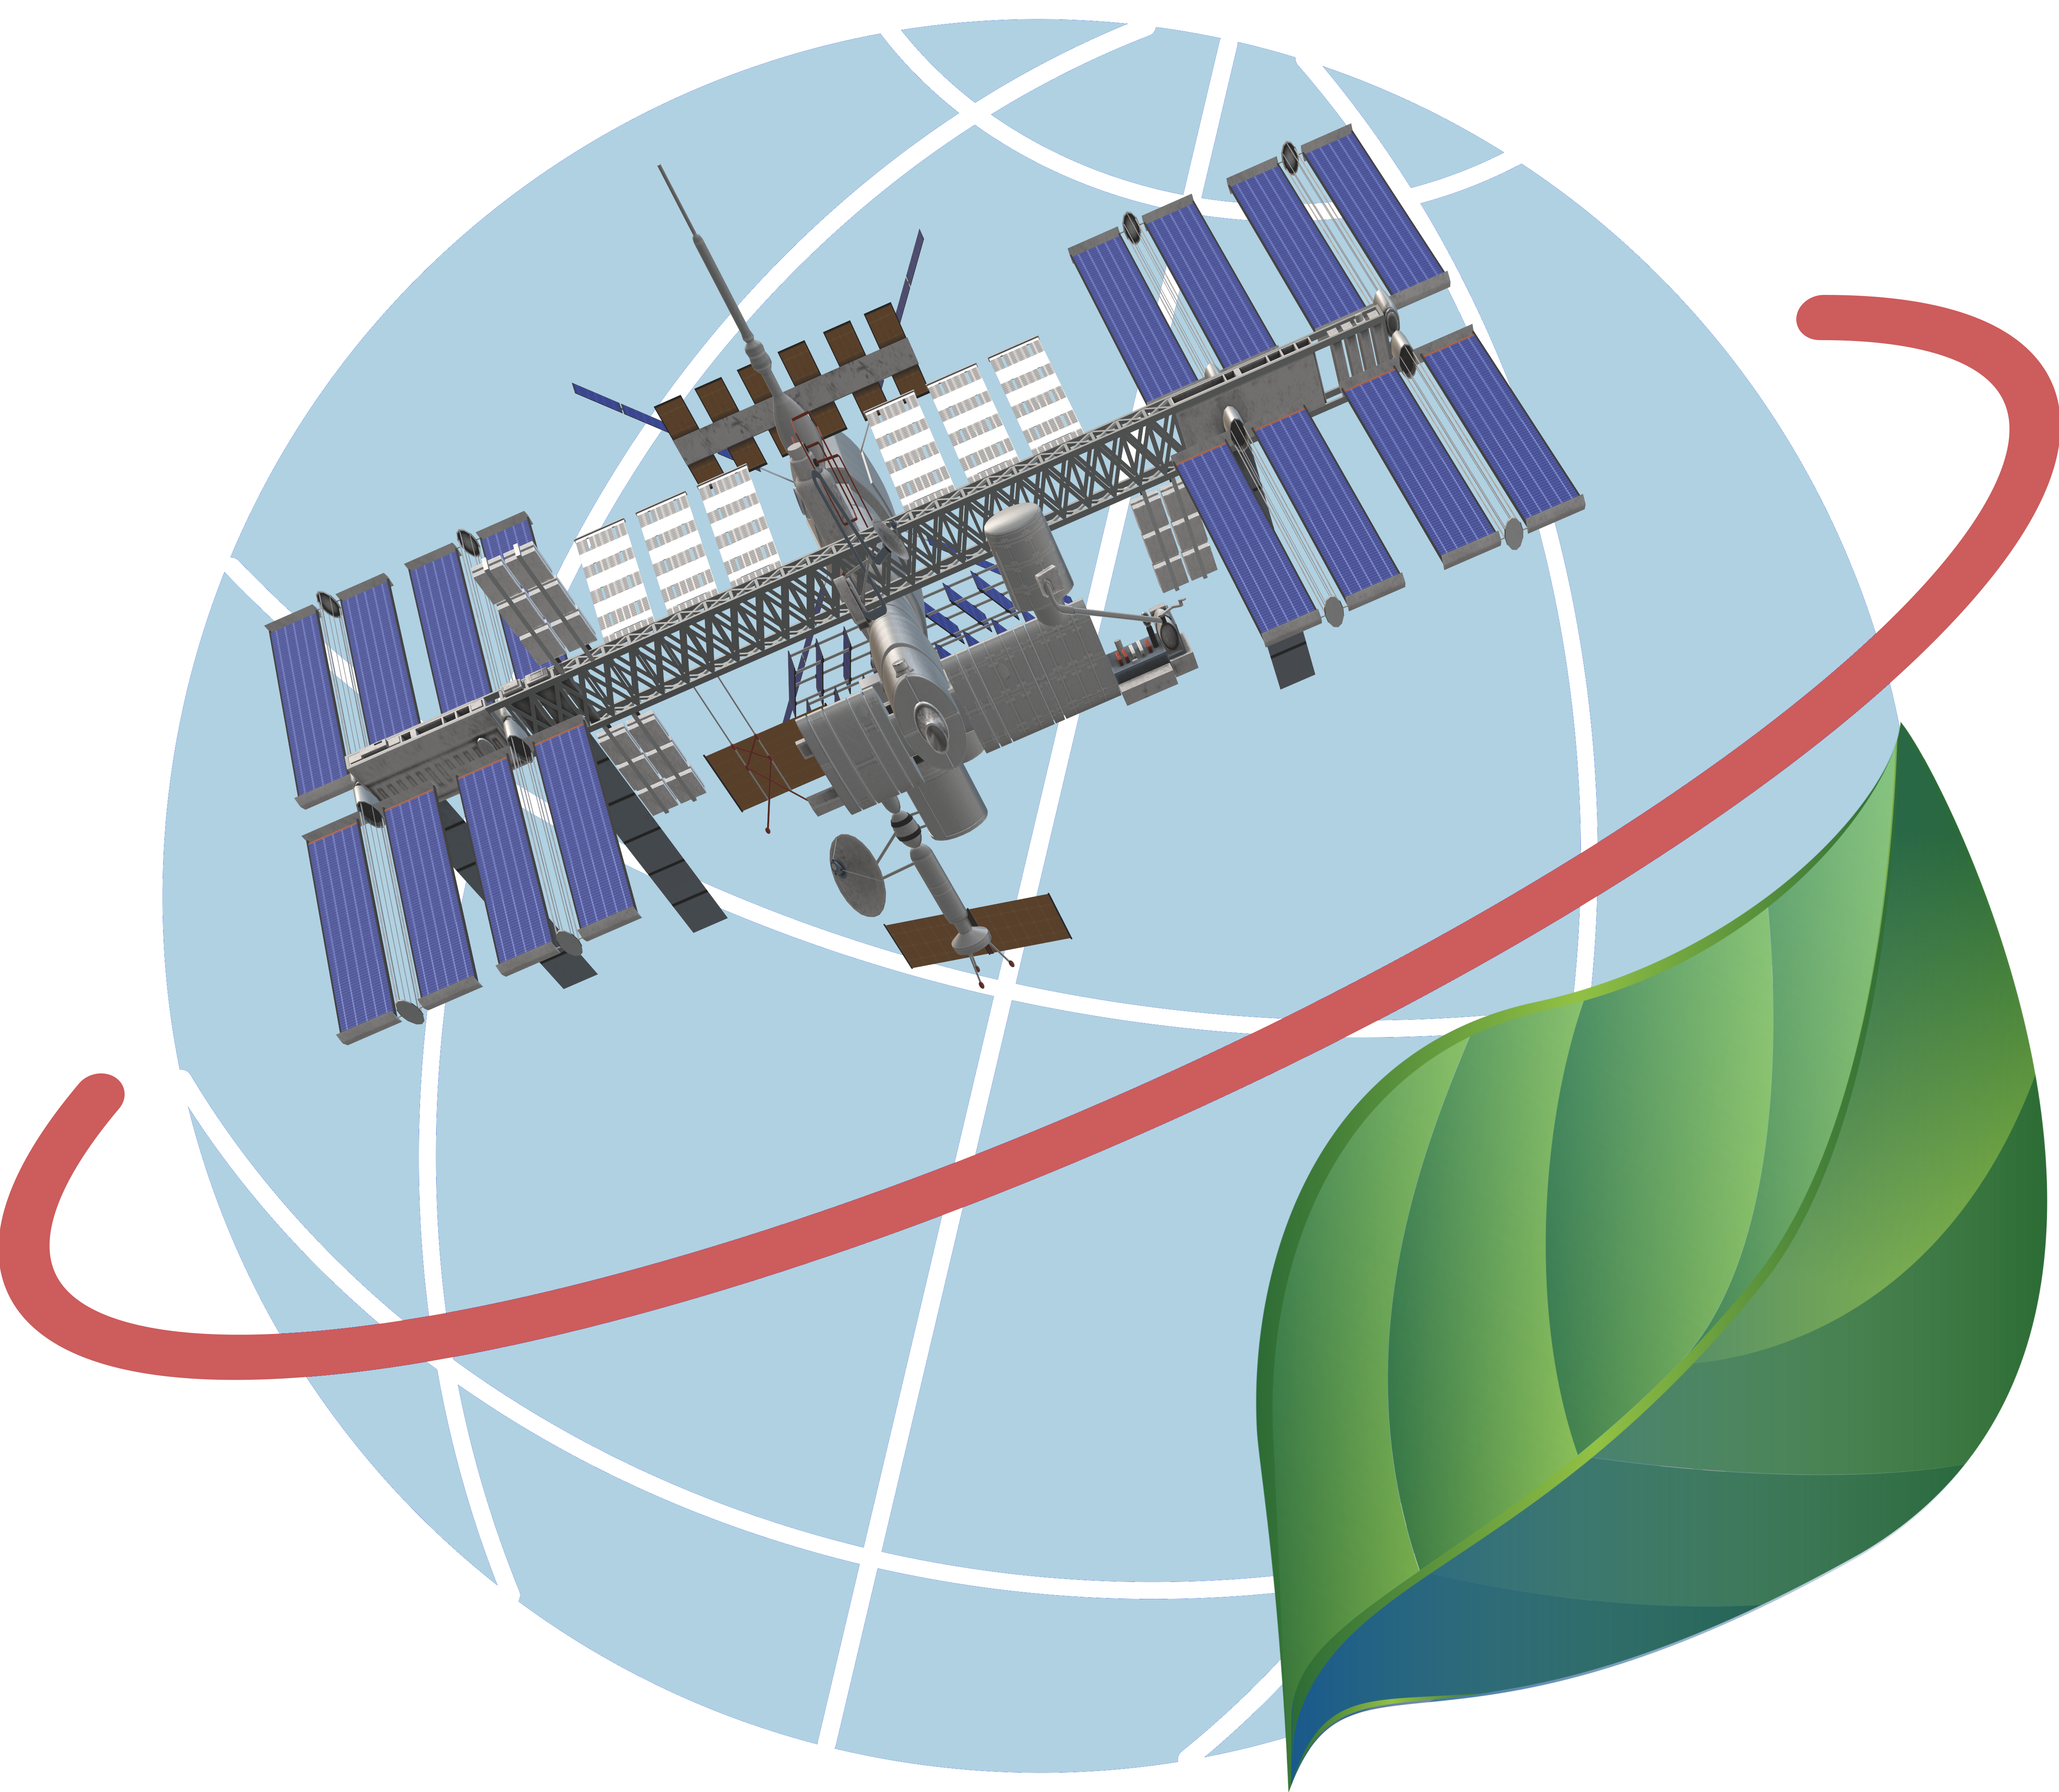
\includegraphics[scale=.125]{ICECREAM_Logo.png}};\end{tikzpicture}}
	%%%%%%%%%%%%%%%%%%%%%%%%%%%%%%%%%%
	
	\noindent\fbox{\begin{minipage}{.9665\textwidth}
			
			\vspace{1em}
			\begin{center}
				\textbf{\Large \underline{Motivation For Today's Tutorial : Upcoming Temperature Competition}}
			\end{center}
			
			\vspace{1 em}
			
			\centerline{
\includegraphics[width=.75\textwidth]{Hometown.png}}
			
			\vspace{1 em}
			
			
			For this and the previous tutorial, our goal is to increase the skills you have in your toolkit when working with the occasionally annoying quirks associated with satellite remote sensing data. Ultimately, we will have an in class competition to see who had the hottest and coldest hometown temperatures, but for now let's talk about one of the biggest cause of headaches for remote sensing researchers: \includegraphics[height=\fontcharht\font`\B]{Clouds.png} . 
			
	\end{minipage}}
	
	\vspace{1 em}

	\section{ECOSTRESS \& Clouds}
	
	ECOSTRESS (like nearly all instruments used for remote sensing) cannot see through the clouds and relies on clear skies to provide reliable observations of land surface temperature. The A$\rho\rho$EEARS database has a few layer options to ensure clouds aren't interfering with an analysis, depending on your goals and timeframes. You may remember that we used the \textit{Cloud\_final} layer in  \href{https://jeremydforsythe.github.io/icecream-tutorials/Tutorial3_AccessingRemoteSensingDataWithAppears/Tutorial3_AccessingRemoteSensingDataWithAppears.pdf}{Tutorial 3's} Death Valley Experiment. This is a newer ``V2'' product that was introduced in late 2022. For data before that or if you are needing more information than simply presence/absence of clouds, ECOSTRESS has alternative metrics available in A$\rho\rho$EEARS:
	
	\begin{tcbraster}[raster columns=3, raster equal height, raster column skip=-.5mm]
		\begin{tcolorbox}[colback=yellow!5!white,colframe=IceCreamLeaf,
			colbacktitle=IceCreamLeaf,title=Cloud\_final]
			\begin{center}
				\includegraphics[width=\columnwidth]{Cloud_final.png}
			\end{center}
			\begin{itemize}[leftmargin=*]
				\item Simple \& straightforward.
				\item Pixels with values = 0 have been determined by the algorithm as ``not cloudy''.
				\item Pixels with values = 1 have been determined by the algorithm as ``cloudy''.
				\item Includes QA Stats for confidence in cloudiness determination, 0 = ``confidently clear'', 1 = ``probably clear'', and 2 =``probably cloudy'', and 3 = ``confidently cloudy''.
				\item Easy to visualize clouds in QGIS.
				\item Only available from late 2022 on!
			\end{itemize}
		\end{tcolorbox}
		\begin{tcolorbox}[colback=yellow!5!white,colframe=IceCreamLeaf, colbacktitle=IceCreamLeaf,title=SDS\_CloudMask]
			\begin{center}
				\includegraphics[width=\columnwidth]{SDS_CloudMask.png}
			\end{center}
			\begin{itemize}[leftmargin=*]
				\item Previous version of \textit{Cloud\_final}.
				\item Not as user-friendly.
				\item Best to visualize through A$\rho\rho$EEARS built-in graphs.
				\item Contains cloud information in addition to the tests used to determine cloudiness.
			\end{itemize}
		\end{tcolorbox}
		\begin{tcolorbox}[colback=yellow!5!white,colframe=IceCreamLeaf,
			colbacktitle=IceCreamLeaf,title=SDS\_QC]
			\begin{center}
				\includegraphics[width=\columnwidth]{SDS_QC.png}
			\end{center}
			\begin{itemize}[leftmargin=*]
				\item Broad quality control.
				\item Not as user-friendly.
				\item Best to visualize through A$\rho\rho$EEARS built-in graphs.
				\item Contains cloud information in addition to other quality metrics regarding missing pixels and atmosphere conditions.
			\end{itemize}
		\end{tcolorbox}
	\end{tcbraster}
	
	\vspace{.25em}
	
	\hrule
	
	\vspace*{.75em}
	
	To showcase the differences in these layers, let's create a new request in A$\rho\rho$EEARS for the Vancouver Island shapefile you drew in the last tutorial (ADD LINK). Let's use the week between Christmas Eve 2022 and New Year's Day 2023.
	
	1. Head over to \href{https://appeears.earthdatacloud.nasa.gov/}{https://appeears.earthdatacloud.nasa.gov/} and sign in.
	
	2. Click the \textit{Extract} dropdown menu to select Area. Next select Start a New Request.
	
	3. Use the screenshot below to set up your request. Name your sample, upload your Vancouver Island \textit{.zip} shapefile, enter \textit{12-24-2022} and \textit{01-01-2023} as start and end dates, and select ECOSTRESS land surface temperature (\textit{SDS\_LST}), \textit{SDS\_QC}, \textit{Cloud\_final}, and \textit{SDS\_CloudMask} as layers. Keep GeoTiff as the format and select \textit{Native Projection} for the projection. Click \textit{Submit}.
	
	\centerline{\includegraphics[width=.75\textwidth]{ExtractVancouver.png}}
	
	4. Use the \textit{Explore} dropdown menu to track the status of your request. 
	
	\vspace{.25em}
	
	\centerline{\includegraphics[width=.75\textwidth]{ExploreRequest.png}}
	
	5. When the request is complete, click on the name of your request to access the layer stats.
	
	6. In the meantime, let's visualize some of the cloud data. I have already accessed the \textit{Cloud\_final} layer for Vancouver Island from 1/1/2023. 
	
	\begin{tcolorbox}[colback=yellow!5!white,title=\textbf{Vancouver Island \textit{Cloud\_final} Layer Files}]
			
		\textbf{Please download these three GeoTIFF files, saving them somewhere logical and accessible, such as the same folder you used for the Vancouver Island shapefile:}
			
		\vspace{-1em}
			
		\begin{itemize}
			\item \href{https://jeremydforsythe.github.io/icecream-tutorials/Tutorial7_CloudyDays/ECO_L2_CLOUD.002_Cloud_final_doy2023001105856_aid0001.tif}{ECO\_L2\_CLOUD.002\_Cloud\_final\_doy2023001105856\_aid0001.tif}
			\item \href{https://jeremydforsythe.github.io/icecream-tutorials/Tutorial7_CloudyDays/ECO_L2_CLOUD.002_Cloud_final_doy2023001123515_aid0001.tif}{ECO\_L2\_CLOUD.002\_Cloud\_final\_doy2023001123515\_aid0001.tif}
			\item \href{https://jeremydforsythe.github.io/icecream-tutorials/Tutorial7_CloudyDays/ECO_L2_CLOUD.002_Cloud_final_doy2023001141155_aid0001.tif}{ECO\_L2\_CLOUD.002\_Cloud\_final\_doy2023001141155\_aid0001.tif}
		\end{itemize}
			
	\end{tcolorbox}
	
	7. Switch over to QGIS, where you should still have your shapefile loaded as a layer. Load these three GeoTIFFs into active layers by double clicking on each in the browser window.
	
	\centerline{\includegraphics[width=.875\textwidth]{Cloud_final_AddLayer.png}}
	
	8. Right click on one of the layers in the \textit{Layer} browser, and select \textit{Properties}.
	
	9. In the panel, make sure \textit{Symbology} is selected.
	
	10. Change \textit{Render type} to \textit{Singleband pseudocolor}, which tells QGIS that we want this layer to be in color.
	
	11. Change \textit{Mode} to \textit{Equal Interval}. Now, we have told QGIS that we want this layer to be to have different colors for each value. 
	
	12. Change \textit{Classes} to \textit{2}. Remember Cloud\_final has only two values. 0 = ``not cloudy'' and 1 = ``cloudy''. Now we can change the color for each value.
	
	13. Right click on Windows/Linux or ctrl-click on Mac for the first value, 0. 
	
	14. Since 0 = ``not cloudy'', lets change this to be completely transparent by sliding the \textit{Opacity} bar all the way to zero. Click \textit{OK} and then right click on Windows/Linux or ctrl-click on Mac for the second value, 1. 
	
	15. If you are feeling particularly dark, make the clouds black by typing ``\#000000'' in the HTML notation box (this is HTML code for black.) Click \textit{OK}.
	
	16. Click \textit{Apply} to apply the color changes to your map.
	
	17. Repeat these steps for the other two Cloud\_final layers. You now have a cloudiness map for New Year's Day 2023 on Vancouver Island.
	
	18. Checking back on our Vancouver Island request in A$\rho\rho$EEARS. If it is ready, you can browse through the different layers shows to see how the quality and cloud metrics work. 
	
	\textbf{Cloud\_final:}
	
	\centerline{\includegraphics[width=.85\textwidth]{Cloud_final_Layer.png}}
	
	\textbf{Cloud\_confidence:}
	\centerline{\includegraphics[width=.85\textwidth]{Cloud_confidence.png}}
	
	\textbf{SDS\_CloudMask:}
	\centerline{\includegraphics[width=.85\textwidth]{SDS_CloudMask_Layer.png}}
	
	\clearpage
	
	\textbf{SDS\_QC:}
	\centerline{\includegraphics[width=\textwidth]{SDS_QC_Layer.png}}
	
	\vspace{.5em}
	
	The layers we have described here start simple and increase in complexity. As a general rule, we suggest using the simplest tools to complete your task. So, if your desired data is after November 2022, stick with the Cloud\_final layer. If it is before November 2022, use the SDS\_CloudMask. Finally, as your interest in remote sensing grows, you can learn more about the SDS\_QC layer in the \href{https://lpdaac.usgs.gov/documents/423/ECO2_User_Guide_V1.pdf}{ECOSTRESS Level 2 Product User Guide.}

	%%%%%%%%%%%%%%%%%%%%%%%%%%%%%%%%%%%%%%%%%%%%%%%%%%%%%%%%%%%%%%%%%%%%%%%%%%%%%%%%%%% Begin End Matter
	
	\vspace{.25em}
	
	\hrule
	
	\vspace{1 em}
	
	\begin{tcolorbox}[colback=yellow!5!white,colframe=IceCreamOrbit,title= \vspace{.2em} \Large Map of the Week Assignments]
		\addcontentsline{toc}{section}{Map of the Week Assignments}
		\large
		\begin{enumerate}
			\item Read about how your choice of colors in maps can be very important in the article: \href{https://theconversation.com/how-rainbow-colour-maps-can-distort-data-and-be-misleading-167159}{How rainbow colour maps can distort data and be misleading.}
			\item Submit a cloudiness map for New Year's Day 2023 for Vancouver Island along with a brief description of your map. Think of it like a caption underneath. Which parts of the island were cloudy that day? Do you see any interesting patterns?
		\end{enumerate}
		
		Submit your map via Canvas before Monday's class.
	\end{tcolorbox}
	
	\vfill
	
	\hrule
	
	\vspace{1em}
	
	\textbf{Recommended Citation:} Forsythe, J.D., G.R. Goldsmith, and J.B. Fisher. 2023. Observing Earth from Above Tutorials. Chapman University. \url{https://jeremydforsythe.github.io/icecream-tutorials/}
	
	\vspace{1em}
	
	This work is supported by funding from NASA ECOSTRESS Mission Grant \#80NSSC23K0309 (I.C.E. C.R.E.A.M.: Integrating Communication of ECOSTRESS Into Community Research, Education, Applications, and Media).
	
\end{document}
